\let\negmedspace\undefined
\let\negthickspace\undefined
\documentclass[journal]{IEEEtran}
\usepackage[a5paper, margin=10mm, onecolumn]{geometry}
%\usepackage{lmodern} % Ensure lmodern is loaded for pdflatex
\usepackage{tfrupee} % Include tfrupee package

\setlength{\headheight}{1cm} % Set the height of the header box
\setlength{\headsep}{0mm}     % Set the distance between the header box and the top of the text

\usepackage{gvv-book}
\usepackage{gvv}
\usepackage{cite}
\usepackage{amsmath,amssymb,amsfonts,amsthm}
\usepackage{algorithmic}
\usepackage{graphicx}
\usepackage{textcomp}
\usepackage{xcolor}
\usepackage{txfonts}
\usepackage{listings}
\usepackage{enumitem}
\usepackage{mathtools}
\usepackage{gensymb}
\usepackage{comment}
\usepackage[breaklinks=true]{hyperref}
\usepackage{tkz-euclide} 
\usepackage{listings}
\usepackage{gvv}                                        
\def\inputGnumericTable{}                                 
\usepackage[latin1]{inputenc}                                
\usepackage{color}                                            
\usepackage{array}                                            
\usepackage{longtable}                                       
\usepackage{calc}                                             
\usepackage{multirow}                                         
\usepackage{hhline}                                           
\usepackage{ifthen}                                           
\usepackage{lscape}
\begin{document}

\bibliographystyle{IEEEtran}
\vspace{3cm}

\title{9.5.3}
\author{AI24BTECH11024-Pappuri Prahladha}
% \bigskip
{\let\newpage\relax\maketitle}

\renewcommand{\thefigure}{\theenumi}
\renewcommand{\thetable}{\theenumi}
\setlength{\intextsep}{10pt} % Space between text and floats


\numberwithin{equation}{enumi}
\numberwithin{figure}{enumi}
\renewcommand{\thetable}{\theenumi}


\textbf{Question:}\\
Find the area of the region bounded by the curves $\brak{x-1}^{2} +y^{2} = 1$ and $ x^{2}+y^{2}  = 1$. 

\hfill (12, 2019)
\\
\textbf{Solution: }\\
\begin{table}[h!]
    \renewcommand{\thetable}{1}
    \centering
    \begin{tabular}[12ptx]{ |c| c|}
\hline\textbf{Term} & \textbf{Description}\\
\hline
$\hat{i}$ and $-\hat{i}$ & Unit vectors along East and West directions \\

\hline
$\hat{j}$ and -$\hat{j}$ & Unit vectors along North and south directions\\
\hline
$\vec{V_{1}}$ or Vector 1 and $\vec{V_{2}}$ or Vector 2 & velocity vectors of Rain and Wind\\
\hline
$\vec{V_{3}}$ or Vector 3 & Resultant velocity vector of Rain and Wind\\
\hline
$\theta$ & Required angle with the horizontal\\
\hline
\end{tabular}
    \caption{Terms used}
    \label{TABLE 1:}
\end{table}\\



The conic parameters for the two circles can be expressed as
\begin{align}
\begin{split}
	\vec{V}_1 &= \myvec{1&0\\0&1},\
	\vec{u}_1 = \myvec{-1\\0},\
	f_1 = 0,
	\\
	\vec{V}_2 &= \myvec{1&0\\0&1},\
	\vec{u}_2 = \myvec{0\\0},\
	f_2 = -1.
\end{split}
	\label{eq:12/8/2/2/vuf}
\end{align}
On substituting from
	\eqref{eq:12/8/2/2/vuf}
	in
	  \eqref{eq:pair-mat-sing-conic-det}, we obtain
\begin{align}
	\mydet{1+\mu & 0 & -1 \\ 0 & 1+\mu & 0 \\ -1 & 0 & -\mu} = 0
\end{align}
yileding
\begin{align}
	\mu= -1.
\end{align}
Substituting 
	\eqref{eq:12/8/2/2/vuf}
in 
	  \eqref{eq:pair-mat-sing-conic},
	  we obtain
\begin{align}
	\vec{x}^\top\myvec{0&0\\0&0}\vec{x} + 2\myvec{-1&0}\vec{x} + 1 &= 0\\
\implies	\myvec{-2&0}\vec{x} &= -1 
\label{eq:12/8/2/2/chord}
\end{align}
Therefore the intersection of the two circles is a line with parameters
\begin{align}
	\vec{m} = \myvec{0\\1},  \vec{h} = \myvec{\frac{1}{2}\\0}.
\end{align}
	The intersection parameters of the 
	chord in 
\eqref{eq:12/8/2/2/chord}
with the 
first circle in \eqref{eq:12/8/2/2/vuf} is obtained from 
\eqref{eq:tangent_roots}
	as
\begin{align}
	\mu_i= \pm\frac{\sqrt{3}}{2}
\end{align}
Hence the point of intersection are
obtained from
	\eqref{eq:chord-pts}
	as
\begin{align}
	\vec{a}_0 = \myvec{\frac{1}{2}\\[1ex]\frac{\sqrt{3}}{2}}, \vec{a}_2 = \myvec{\frac{1}{2}\\[1ex]-\frac{\sqrt{3}}{2}}.
\end{align}
The desired area of region is given as
\begin{multline}
	2\brak{\int_{0}^{\frac{1}{2}} \sqrt{1-\brak{x-1}^2}dx + \int_{\frac{1}{2}}^{1} \sqrt{1-x^2}dx}\\
		=2\sbrak{\frac{1}{2}\brak{x-1}\sqrt{1-\brak{x-1}^2}+\frac{1}{2}\sin^{-1}\brak{x-1}}_{0}^{\frac{1}{2}}\\
		 +2\sbrak{\frac{x}{2}\sqrt{1-x^2}+\frac{1}{2}\sin^{-1}x}_{\frac{1}{2}}^{1}
	= \frac{2\pi}{3}-\frac{\sqrt{3}}{2}=1.22837
\end{multline}
 \begin{figure}[h!]
   \centering
   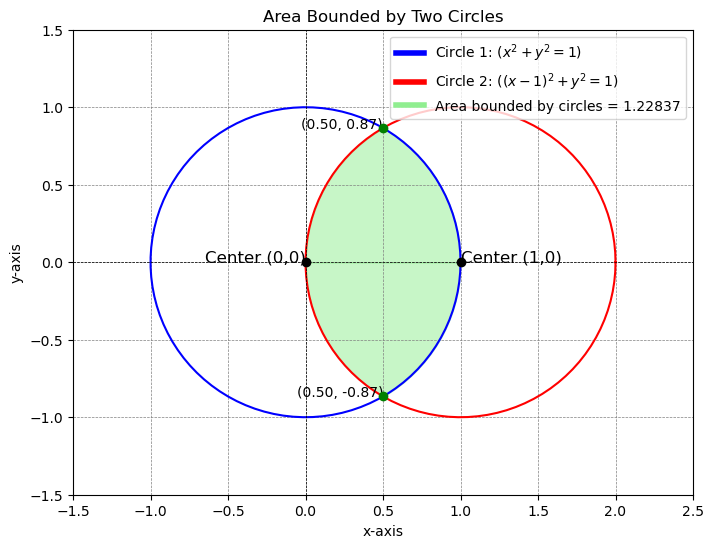
\includegraphics[width=0.7\linewidth]{figs/figure1.png}
   \caption{Plot showing area bounded by the circles}
   \label{stemplot}
\end{figure}
\end{document}
